\documentclass{standalone}
\usepackage{pgfplots}
\usepackage{pgfplotstable}
\pgfplotsset{compat=1.17}

\begin{document}
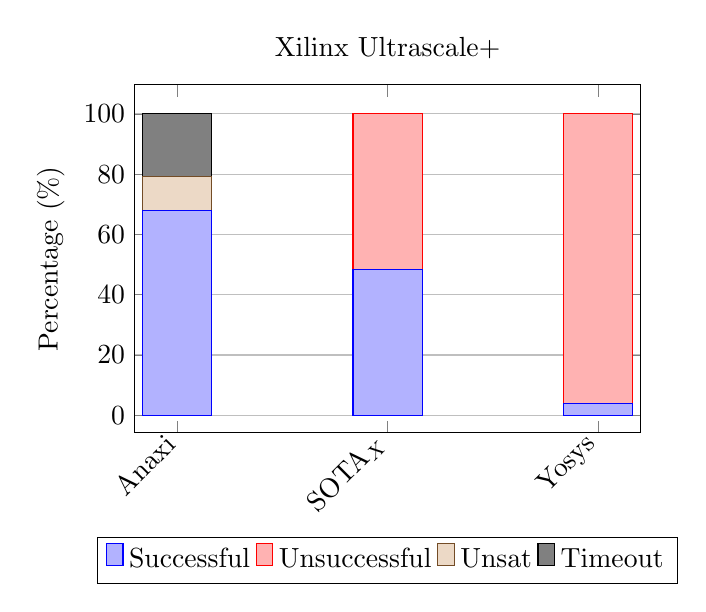
\begin{tikzpicture}
  \pgfplotstableread[col sep=comma]{
,tool,num_experiments,num_successful,num_unsuccessful,num_lr_unsat,num_lr_timeout,total_experiments,percentage_successful,percentage_unsuccessful,percentage_lr_unsat,percentage_lr_timeout
0,Anaxi,990,673,0,110,207,990,67.97979797979798,0.0,11.11111111111111,20.909090909090907
1,SOTA$_X$,990,480,510,0,0,990,48.484848484848484,51.515151515151516,0.0,0.0
2,Yosys,990,38,952,0,0,990,3.8383838383838382,96.16161616161617,0.0,0.0
% 3,Anaxi-Lattice,264,216,0,0,48,264,81.81818181818183,0.0,0.0,18.181818181818183
% 4,SOTA Lattice,264,88,176,0,0,264,33.33333333333333,66.66666666666666,0.0,0.0
% 5,Yosys-Lattice,264,44,220,0,0,264,16.666666666666664,83.33333333333334,0.0,0.0
  }\datatable

  \begin{axis}[
    title = Xilinx Ultrascale+,
    ybar stacked,
    bar width = 25pt,
    width=8cm,
    height=6cm,
    ylabel={Percentage (\%)},
    symbolic x coords={Anaxi,SOTA$_X$,Yosys},
    xtick=data,
    % nodes near coords,
    % nodes near coords align={vertical},
    legend style={
      at={(0.5,-0.3)},
      anchor=north,
      legend columns=-1,
    },
    x tick label style={rotate=45,anchor=east},
    ymajorgrids,
    try min ticks = 5
  ]
    \addplot table[y=percentage_successful,x=tool] {\datatable};
    \addplot table[y=percentage_unsuccessful,x=tool] {\datatable};
    \addplot table[y=percentage_lr_unsat,x=tool] {\datatable};
    \addplot table[y=percentage_lr_timeout,x=tool] {\datatable};
    \legend{Successful,Unsuccessful,Unsat,Timeout}
  \end{axis}
\end{tikzpicture}
\end{document}
